\chapter{Análise dos Resultados}
O ePuppy continua em desenvolvimento com duas partes do projeto, a {\it front-end} e {\it back-end}. Cada parte envolvida está encarregada de dar prosseguimento ao andamento do sistema. O {\it Front-end} cuida da parte gráfica, enquanto o {\it Back-end} cuida do controle e da lógica por trás do software. Por enquanto o projeto ainda não se encontra hospedado, por se encontrar em fase de testes lógicos.
\\
\indent
O ePuppy conta com segurança de permissão, que garante que os usuários só naveguem no sistema através da interface gráfica, impedindo alguma falha de segurança da informação, caso os mesmos tentem navegar pela url impedindo a entrada caso não encontrem-se logados.

\begin{figure}[h!]
	\center	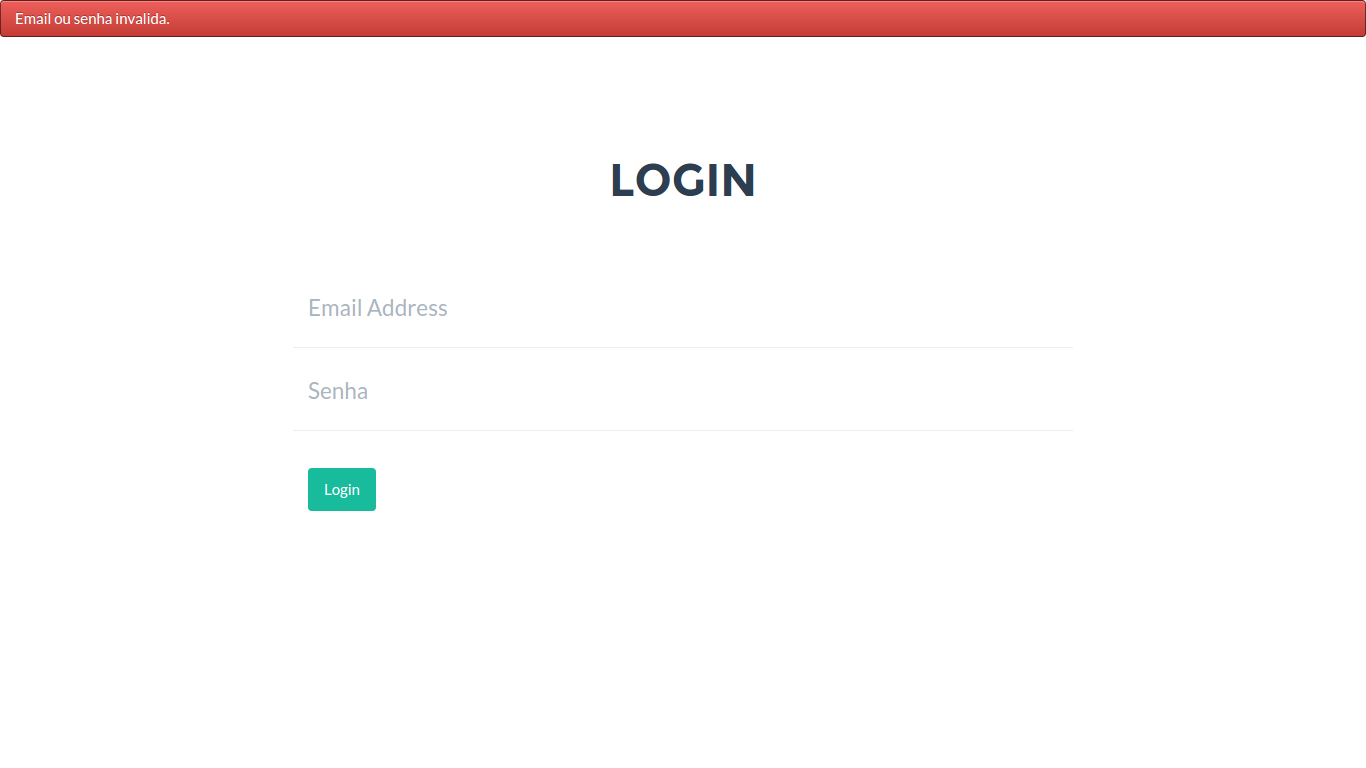
\includegraphics[scale=0.33
	]{imagens/errologin}
	\caption{Login com falha na autenticação}
	Fonte: Autoria Própria.
	\label{Rotulo}
\end{figure}

A página inicial do projeto conta com uma fácil navegação e simplicidade, assim otimizando o tempo do usuário durante o {\it login}. Dentro desta página há recursos como cadastrar, desenvolvedores e as funcionalidades que poderão ser encontradas através da rolagem da página ou escolhidos no menu superior, fazendo com que o site inicial seja completamente integrado e interativo.
\begin{figure}[h!]
	\center	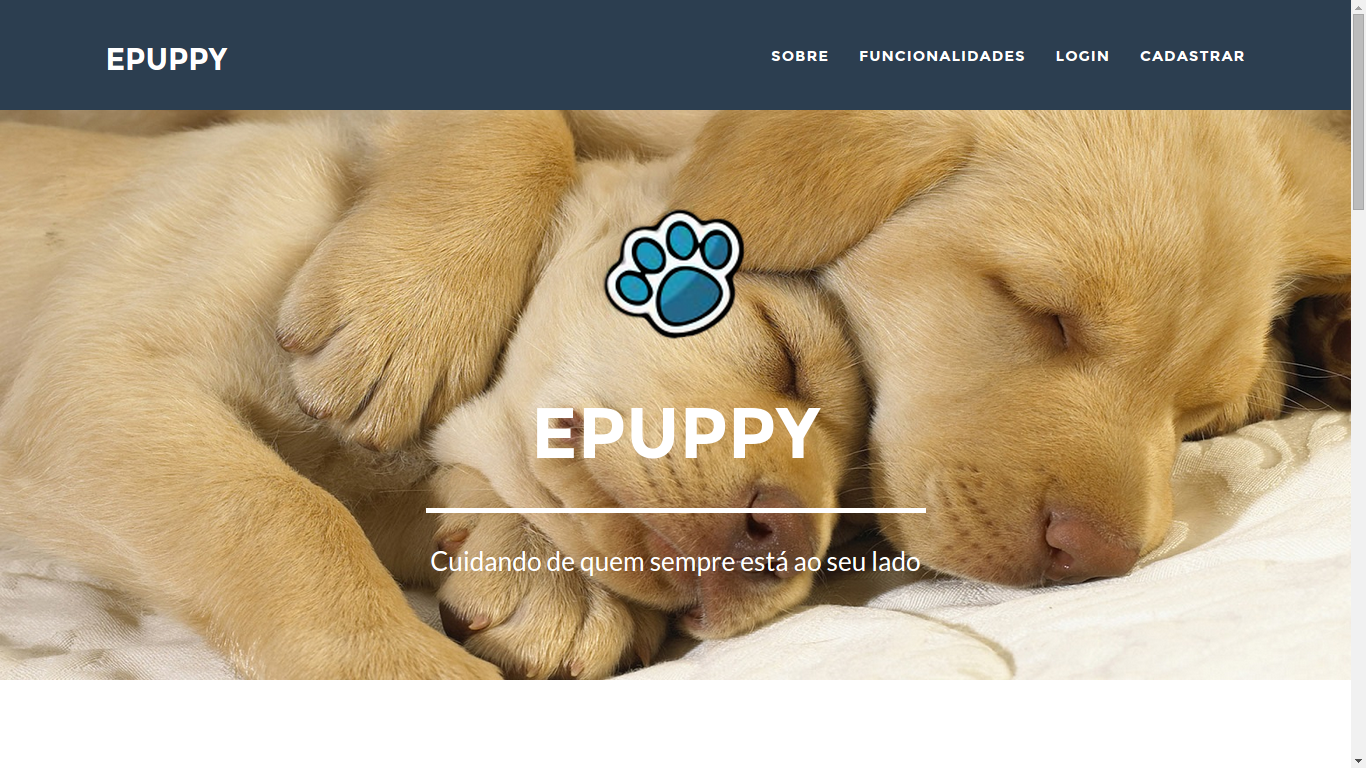
\includegraphics[scale=0.26
	]{imagens/principal}
	\caption{Página home do ePuppy}
	Fonte: Autoria Própria.
	\label{Rotulo}
\end{figure}
\begin{figure}[h!]
	\center	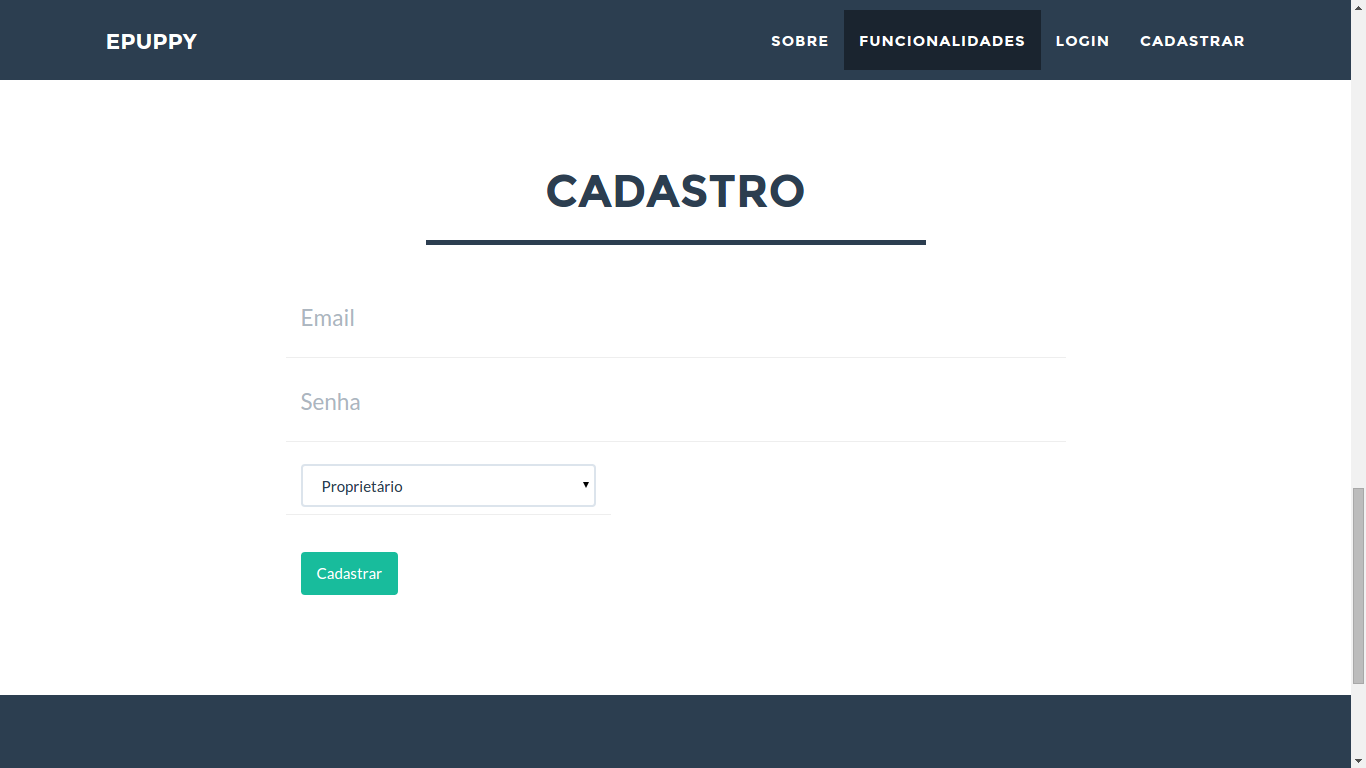
\includegraphics[scale=0.26
	]{imagens/cadastro}
	\caption{Página de cadastro do ePuppy}
	Fonte: Autoria Própria.
	\label{Rotulo}
\end{figure}

O projeto que teve início em Julho do ano passado e sua principal característica é a integração dos proprietários com clínicas e veterinários, reunindo-os em um único espaço, fazendo disto uma grande rede social interligada, facilitando o cuidado de seu(s) {\it pet}(s). Ao se cadastrar no ePuppy, os proprietários terão direito a adicionar seus animais, seus momentos com ele e entrar com o pedido de coleiras personalizadas, para que em casos de fuga ou perca, este possa ser facilmente encontrado. Caso o usuário não queira adquirir as coleiras personalizadas, o sistema disponibilizará o {\it QR Code} separadamente, podendo assim ser facilmente impressa conforme o desejo do proprietário.
\begin{figure}[h!]
	\center	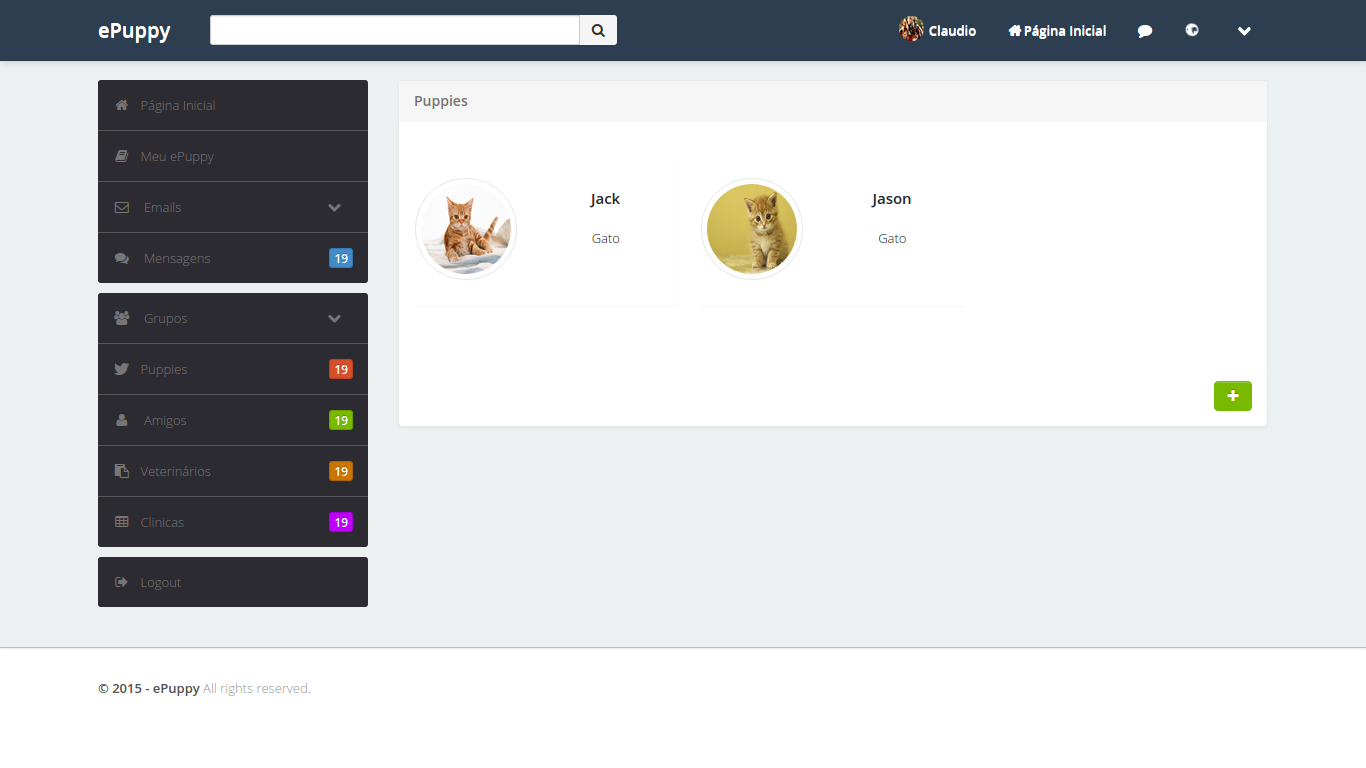
\includegraphics[scale=0.22
	]{imagens/animais1}
	\caption{Página home dos animais de estimação}
	Fonte: Autoria Própria.
	\label{Rotulo}
\end{figure}
\begin{figure}[h!]
	\center	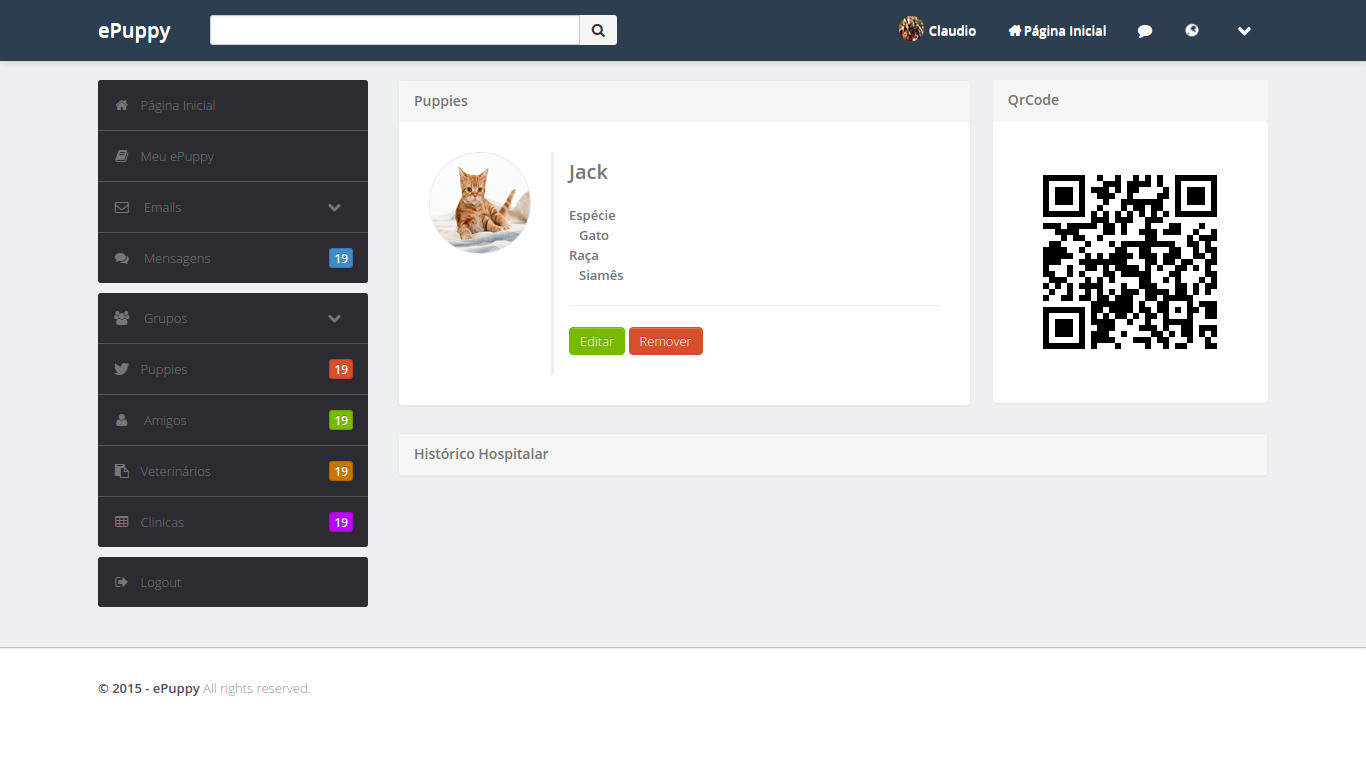
\includegraphics[scale=0.22
	]{imagens/animais2}
	\caption{Página de detalhes dos animais de estimação}
	Fonte: Autoria Própria.
	\label{Rotulo}
\end{figure}

É importante destacar que toda a navegação dentro do ePuppy contém o mesmo padrão de navegabilidade e, portanto faz com que as funções sejam notadas claramente pelo usuário e este consiga passar entre todas as {\it urls} do sistema sem precisar de explicação alguma. O usuário poderá ver todos os detalhes de sua conta na sua página principal, na qual, mostrará todos dos seus animais, grupos, amigos e suas principais postagens.

\begin{figure}[h!]
	\center	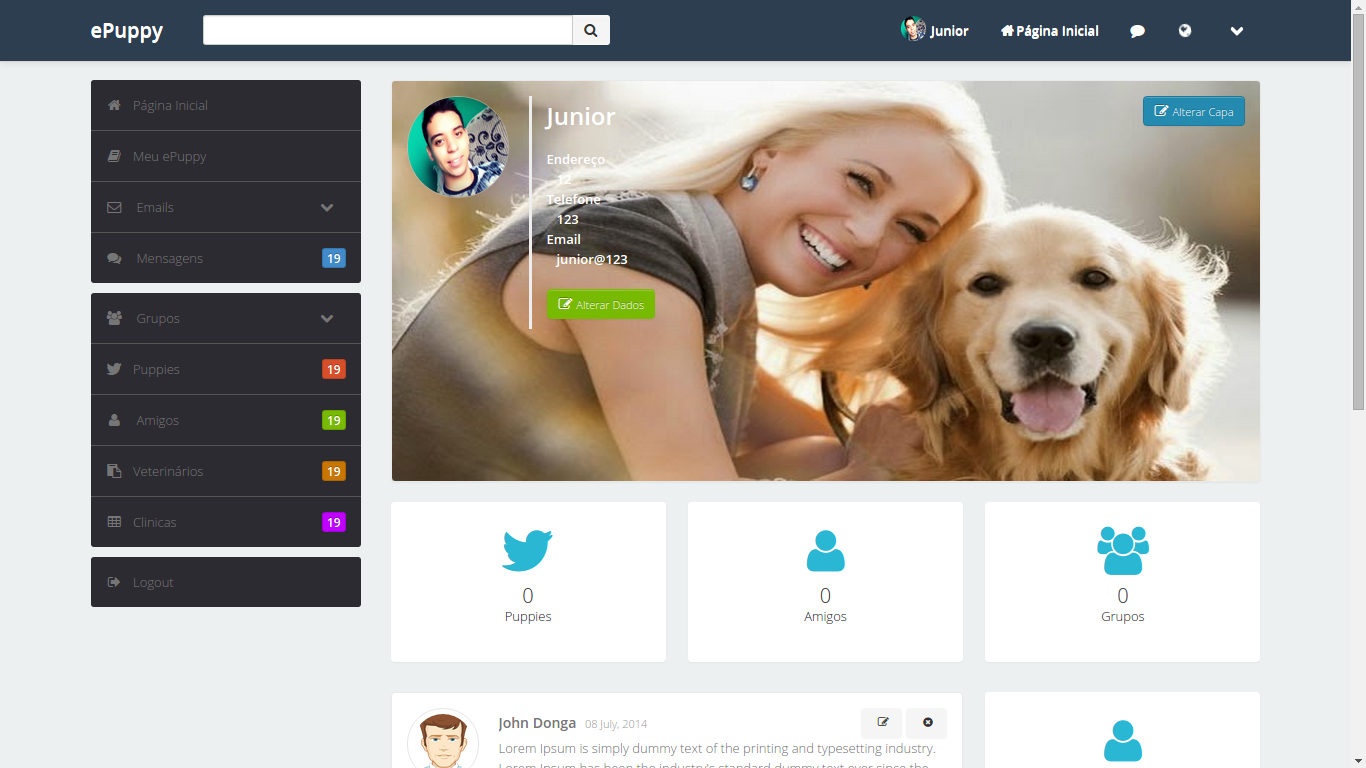
\includegraphics[scale=0.33
	]{imagens/perfil}
	\caption{Perfil do usuário}
	Fonte: Autoria Própria.
	\label{Rotulo}
\end{figure}

A vantagem de utilizar o ePuppy em vez de algum outro programa é a interação que ele propõe dentro do âmbito dos cuidados do animal. Por ser uma grande rede interligada permite que funções de segurança também sirvam para saúde. As coleiras personalizadas, além da função supracitada também servirão para o atendimento dos animais, a medida que o veterinário permitido pelo dono do {\it pet}, pode verificar todo o histórico hospitalar deste, identificando assim, quem fez determinada consulta, a descrição desta e os medicamentos ou cirurgias passadas a estes.

